% Nature Communications submission — "Large language models in psychology" Collection
% Deadline: 15 Sept 2026 — https://www.nature.com/collections/badbafeeca
% Uses the official Springer Nature LaTeX template (sn-jnl.cls, v3.1) with the
% sn-nature class option, which is specifically for Nature Portfolio journal
% submissions. Downloaded from the official Springer Nature template mirror
% (godkingjay/springer-nature-latex-template, matches the sn.pub author-support zip).
% Bibliography style: sn-nature.bst (Nature Portfolio reference style).
%
% NC structure requirements gathered from their submission pages: structured
% abstract <=200 words, Intro/Results/Discussion/Methods, refs <=70 (guideline),
% single-PDF initial submission, mandatory code-availability statement.

\documentclass[pdflatex,sn-nature]{sn-jnl}

\usepackage{graphicx}
\usepackage{booktabs}
\usepackage{multirow}
\usepackage{amsmath,amssymb,amsfonts}
\usepackage{amsthm}
\usepackage{hyperref}
\usepackage{url}

\raggedbottom

\begin{document}

\title[psychscanner]{Beyond predictive benchmarks: infrastructure for hypothesis-driven cognitive testing of large language models}

% Names, order, and affiliations verified directly from the title page of
% arXiv:2607.29093 (metasignal, same author team minus Odegaard) — quoted
% verbatim, not inferred. Corresponding author email matches CITATION.cff.
\author*[1]{\fnm{Saurabh} \sur{Ranjan}}\email{ranjan.saurabh@outlook.com}
\author[2]{\fnm{Konstantina} \sur{Sokratous}}
\author[3]{\fnm{Mukesh} \sur{Makwana}}

\affil*[1]{\orgname{University of Florida}, \orgaddress{\city{Gainesville}, \state{FL}, \country{USA}}}
\affil[2]{\orgname{University of Missouri}, \orgaddress{\city{Columbia}, \state{MO}, \country{USA}}}
\affil[3]{\orgname{Brown University}, \orgaddress{\city{Providence}, \state{RI}, \country{USA}}}

\abstract{Large language models are increasingly evaluated as psychological
subjects, but NeuroAI and psychology apply incompatible standards:
predicting responses to naturalistic stimuli versus manipulating controlled
stimuli to test falsifiable, mechanism-level hypotheses. No infrastructure
exists for running the second kind of study at the scale quantitative
psychology expects, so researchers hand-build prompt construction, memory
management, and persona conditioning for every task and model.
We introduce psychscanner, an open-source framework in which a researcher
authors a cognitive or survey task once, as a declarative task card, and
runs it across memory architectures, persona manipulations, feedback
regimes, and model families without rewriting any mechanics. A
three-armed bandit task run through three agent architectures found none
produced explore-then-exploit behaviour, with instruction-following
collapse under structured feedback as the dominant effect. A 480-trial
factorial replication of a classic imagery paradigm found persona
conditioning had no measurable effect on vividness ratings, but single-turn
prompting returned an identical rating on every trial, a response-degeneracy
artifact invisible to aggregate benchmark scores. Because every model
backend implements one interface, the same task cards also capture
internal activations: linear probes recover an internal board-state
representation in a trained toy transformer, placing behavioural and
mechanistic testing in one harness.}

% NC convention: no citations/subheadings inside \abstract (kept clean above).
% Word count (verified by tools/count_abstract.py): 196/200.

\keywords{cognitive testing, large language models, task-based evaluation, experimental psychology, reproducible evaluation}

\maketitle

\section{Introduction}\label{sec:intro}

Large language models are increasingly evaluated as objects of
psychological inquiry \citep{hagendorff2023machinepsych,
binz2023gpt3cogpsy}, but the communities doing this evaluation disagree
about what counts as evidence. NeuroAI typically evaluates a model by how
well it predicts behavioural and neural responses to naturalistic stimuli,
treating out-of-sample predictive variance as the mark of success
\citep{binz2025foundation}. Psychology instead evaluates a model by how
well it accounts for the effect of systematically manipulating a
controlled, artificial stimulus to test a specific, falsifiable hypothesis
about a specific mechanism \citep{bowers2023deepproblems}. A model can
predict naturalistic data well while getting the underlying mechanism
wrong, and a model tuned to a controlled manipulation may generalize
poorly outside it — the two standards are not interchangeable, and recent
work has framed this as a live, unresolved methodological disagreement
rather than a settled question: a 2026 Cognitive Computational Neuroscience
Generative Adversarial Collaboration sets researchers who evaluate models
by predictive fit to naturalistic stimuli against researchers who evaluate
models by their account of controlled, manipulation-driven effects, and
finds no consensus resolution \citep{gac2026neuroai}. The disagreement is
concrete, not abstract: a 2026 preprint argues that Centaur
\citep{binz2025foundation} — the very foundation model just cited for
NeuroAI's predictive successes — mistakes predictive power for explanatory
power \citep{bowers2026centaurcritique}, and even its critics hold that
manipulation-based testing should complement rather than replace predictive
modelling \citep{gac2026discussion}, the complement this paper builds for
large language models.

Applying psychology's side of this methodology to large language models at
scale — systematically manipulating one factor (memory, persona, feedback,
stimulus modality) across many models and replications, the way a
cognitive psychology lab would run a study — currently has no dedicated
infrastructure: prompt construction, response parsing, state management,
and persona conditioning are typically hand-built from scratch for every
new task and model family, which makes systematic, multi-condition
replication impractical. We introduce \textbf{psychscanner}, an
open-source framework that closes this gap: a researcher authors a
controlled cognitive or survey task once, as a declarative task card, and
runs it across memory conditions, persona manipulations, feedback regimes,
and model families without rewriting the underlying mechanics — the
missing methodological toolkit for asking manipulation-based, falsifiable
questions about large language model cognition at the scale quantitative
psychology expects.

Existing behavioural instruments for this purpose — benchmarks such as
PsychoBench \citep{huang2024psychobench}, task ontologies such as the
Cognitive Atlas \citep{poldrack2011cogatlas}, and the methodological
guidance now being formalized for treating models as psychological
simulators \citep{lin2025simulators} — give the enterprise structure and
coverage targets, but share one limit: they describe what a model does
without opening it to ask why. That limit is consequential, because the
behavioural divergences this literature keeps surfacing are exactly the
ones whose cause is unclear. Two studies run on earlier versions of the
framework reported here illustrate the pattern: model source-monitoring
accuracy degrades under conversational delay in a way that tracks active
rather than aggregate parameter count \citep{ranjan2026reality}, and model
imagination-vividness ratings collapse into a degenerate single-cluster
network topology where three geographically distinct human populations show
robust community structure \citep{ranjan2025psychological}. Both findings
describe behaviour and stop there.

We therefore designed psychscanner so that the layer which chooses
\emph{which model executes a trial} is a single, swappable interface, and
then implemented backends behind that interface that additionally capture
the model's internal activations for every trial. This is what makes the
framework more than a prompting harness: the three dominant
mechanistic-interpretability methods have direct neuroscience analogues —
linear probing of internal activations is the same operation as neural
decoding from recorded population activity
\citep{li2023othello}; causal tracing, in which an activation is corrupted
and the site that restores correct behaviour is identified, is the
artificial-network analogue of a lesion or reversible-inactivation study
\citep{meng2022rome}; and activation steering along an extracted direction
is the analogue of stimulation along an identified pathway
\citep{chen2025personavectors,burns2023ccs}. Because these run through the
same task cards, persona conditioning, and memory conditions used for the
behavioural experiments, a manipulation that previously yielded only
response differences now also yields paired activation captures, with no
separate extraction pipeline to write. We treat internal activations as a
complement to behavioural measurement rather than a replacement for it:
mechanistic interpretability's own recent self-assessment favours pragmatic
proxy tasks over ambitious reverse-engineering \citep{nanda2025pragmatic},
and a clinical-triage study found that near-perfect internal
representations (98.2\% AUROC from linear probes) did not translate into
corrected model output (steering fixed only 20\% of missed errors)
\citep{basu2026actionability}.

\section{Results}\label{sec:results}

\subsection{Framework architecture}\label{sec:results-arch}

Figure~\ref{fig:blueprint} gives the component structure of the released
package (v0.3.0). A run traverses a fixed spine — the researcher-authored
task card and persona files are resolved into an \texttt{ExpCard}, expanded
into one system message per design cell and one message per trial, executed
by \texttt{TaskRunner} against a configured agent, and validated and written
to disk — while four seams remain open for the researcher: response parsers,
model providers, agent architectures, and trial-level feedback. The
experimental factors a psychologist would want to manipulate are all
declarations on the card or the \texttt{ExpCard} rather than code paths, and
the model provider seam is what carries the interpretability backends
(\S\ref{sec:results-interp}). Six demonstration modules exercise this
feature surface end-to-end on real model calls; the two with complete
behavioural data are reported below, alongside the interpretability
validation.

\begin{figure}[h]
\centering
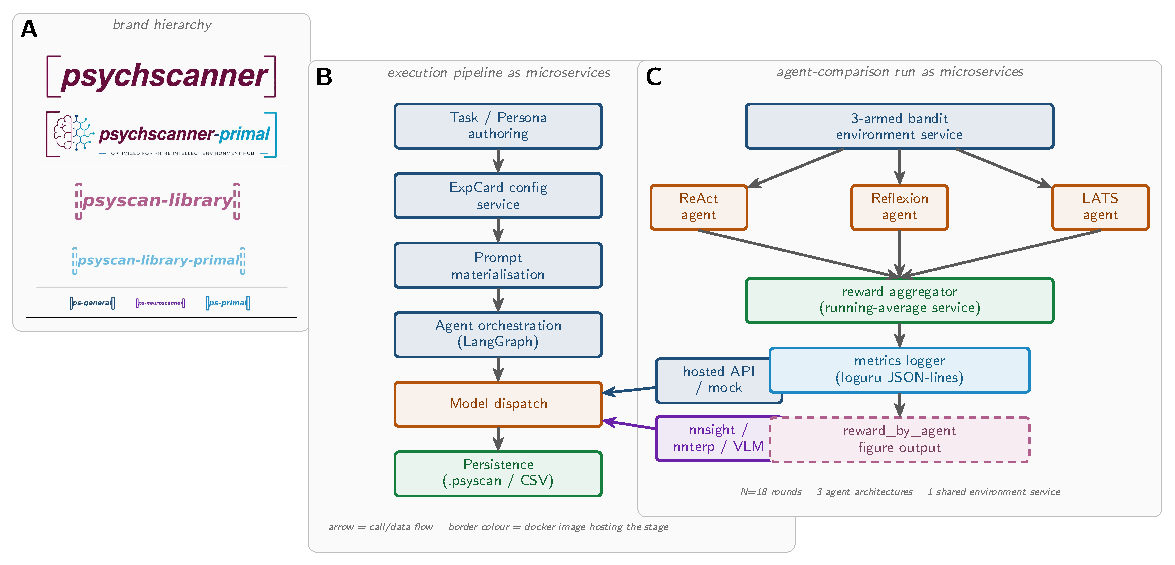
\includegraphics[width=\textwidth]{../figures/figure1_composite.pdf}
\caption{The PsychScanner project as a microservices system. (A) Brand
hierarchy: the two framework repositories (psychscanner,
psychscanner-primal), their companion vetted task/experiment-card
libraries (psyscan-library, psyscan-library-primal), and the three
published Docker images (\texttt{ps-general}, \texttt{ps-neuroscanner},
\texttt{ps-primal}). (B) The single-run execution pipeline of \S
\ref{sec:results-behav}, redrawn as a service pipeline; box border colour
marks which Docker image hosts each stage. (C) The multi-agent bandit
comparison behind Fig.~\ref{fig:bandit}, redrawn the same way: one shared
environment service, three interchangeable agent services, and a
reward-aggregation/logging path terminating in that figure.}
\label{fig:composite}
\end{figure}

\begin{figure}[p]
\centering
\includegraphics[height=0.92\textheight,width=\textwidth,keepaspectratio]{../figures/psychscanner_blueprint.pdf}
\caption{Component blueprint of psychscanner v0.3.0. Blue: the core
execution path traversed by every run. Orange, dashed: the four
researcher-facing extension seams. Purple: the interpretability backends,
which reach the rest of the framework through the same
\texttt{BaseChatModel} interface as every hosted-API backend. Green: on-disk
artifacts. Every label is a symbol in the released package.}
\label{fig:blueprint}
\end{figure}

\subsection{Behavioural manipulations}\label{sec:results-behav}

A 3-armed bandit task run through three
agent architectures (a bare single-call baseline, a generate/reflect loop,
and a plan/execute/validate loop) via a single \texttt{custom\_agent=}
argument found none produced textbook explore-then-exploit behaviour
(baseline: 16.14 total reward, 0\% optimal-arm picks; self-reflection:
14.14, 16.7\% optimal; plan/execute/validate: 12.14, 0\% optimal;
$N{=}18$ rounds, demonstration-scale, not a powered study); the dominant
effect was instruction-following collapse under structured JSON feedback on
an 8B-parameter model, not a clean architecture comparison
(Fig.~\ref{fig:bandit}, Table~\ref{tab:bandit}).

\begin{figure}[h]
\centering

\includegraphics[width=0.7\textwidth]{../figures/reward_by_agent.png}
\caption{Running average reward by agent architecture across the 3-armed
bandit task (Demo 01). The optimal arm's true mean (6.0) is shown as a
dashed reference line; none of the three architectures approaches it.}
\label{fig:bandit}
\end{figure}

\begin{table}[h]
\centering
\caption{Demo 01 per-agent summary. $N=18$ rounds total (6 rounds
$\times$ 3 architectures), demonstration-scale, not a powered study.}
\label{tab:bandit}
\begin{tabular}{@{}lccc@{}}
\toprule
Agent architecture & Total reward & Mean reward/round & \% optimal-arm picks \\
\midrule
Baseline (single-call) & 16.14 & 2.69 & 0\% \\
Self-reflection & 14.14 & 2.36 & 16.7\% \\
Plan/execute/validate & 12.14 & 2.02 & 0\% \\
\bottomrule
\end{tabular}
\end{table}

\textbf{[PLACEHOLDER: paired-associate recall across
memory/feedback conditions; BFI-44 persona $\times$ memory survey;
vision-language accuracy under reward/accuracy feedback; and persona-vector
extraction and steering — design complete (see Methods), quantitative
results pending full data collection.]} A completed extended factorial replication
of the persona/imagery paradigm (VVIQ-16, Supplementary Information S1.1,
$n=480$ trials) found no measurable effect of persona conditioning on
vividness ratings (WEIRD $3.69\pm0.88$ vs.\ non-WEIRD $3.70\pm0.89$), but a
strong memory-condition effect: the persona-conditioned single-turn
condition returned a constant rating of 4 on all 160 trials (SD~$=0$),
whereas the trial-chain
condition's ratings spanned the full 1--5 range ($3.02\pm1.28$;
Fig.~\ref{fig:vviq}, Table~\ref{tab:vviq}). Further extended factorial designs
beyond the six core demos are described in Supplementary Information
Sections S1--S4.

\begin{figure}[h]
\centering

\includegraphics[width=\textwidth]{../figures/trial_trajectory.png}
\caption{VVIQ-16 vividness ratings by trial, memory condition, and
persona (Supplementary Information S1.1). \texttt{item\_ST}
(single-turn) is flat at rating 4 for every trial in both personas;
\texttt{trial\_Cv} shows genuine item-to-item variation.}
\label{fig:vviq}
\end{figure}

\begin{table}[h]
\centering
\caption{VVIQ-16 mean vividness rating ($\pm$SD) by memory condition,
pooled across personas ($n=160$ trials/condition). SD~$=0$ under
\texttt{item\_ST} indicates every trial returned an identical rating.}
\label{tab:vviq}
\begin{tabular}{@{}lcc@{}}
\toprule
Memory condition & Mean vividness & SD \\
\midrule
item\_ST (single-turn) & 4.00 & 0.00 \\
task\_Cv (episodic-chain) & 4.06 & 0.24 \\
trial\_Cv (trial-chain) & 3.02 & 1.28 \\
\bottomrule
\end{tabular}
\end{table}

\subsection{Activation capture through the same
interface}\label{sec:results-interp}

To test whether the model-provider seam in Fig.~\ref{fig:blueprint} really
does carry mechanistic work without a parallel pipeline, we reproduced the
Othello-GPT result \citep{li2023othello} end-to-end through it. A
CPU-tractable toy transformer (4 layers, $d_{\text{model}}=64$, 4 heads)
was trained for 12 epochs on 4,000 games of legal-move sequences only, with
board state never shown during training, and then linearly probed for
board-state decodability at each residual-stream layer on 400 held-out
games (Methods, \S\ref{sec:methods-interp}). Legality checking on the
trained model (728 boundary steps) placed a mean probability mass of 0.998
on legal moves against a random baseline of 0.75, confirming the model had
learned the task before its internals were probed.

Board-state decodability is near the shuffled-label baseline at layer 0
(0.423 vs.\ 0.140) and jumps above 0.93 from layer 1 onward
(Table~\ref{tab:othello}), the same qualitative layer-wise pattern the
original study reported, obtained here on a model we trained ourselves
rather than a reused checkpoint, through the infrastructure built for the
behavioural experiments above.

\begin{table}[h]
\centering
\caption{Linear-probe accuracy for an internal board-state representation
by residual-stream layer, in a toy transformer trained only on legal-move
sequences. The shuffled-label baseline is computed identically at each
layer, to control for probe capacity alone recovering structure.}
\label{tab:othello}
\begin{tabular}{@{}lccc@{}}
\toprule
Layer & Probe accuracy & Shuffled-label baseline & Above baseline \\
\midrule
0 & 0.423 & 0.140 & +0.283 \\
1 & 0.941 & 0.148 & +0.793 \\
2 & 0.953 & 0.149 & +0.804 \\
3 & 0.931 & 0.141 & +0.790 \\
\bottomrule
\end{tabular}
\end{table}

\textbf{[PLACEHOLDER: the two remaining planned reproductions — causal
tracing and rank-one editing \citep{meng2022rome}, and contrast-consistent
search \citep{burns2023ccs} — are implemented as designs but have not been
run, and the persona-vector extraction and steering experiment
\citep{chen2025personavectors} has no collected data as of this draft. The
claim that this backend is validated as a general-purpose probing platform
is therefore currently supported by one of three planned reproductions.]}

\section{Discussion}\label{sec:discussion}

The VVIQ-16 result is the clearest evidence so far for the methodological
claim in the Introduction. A naturalistic or aggregate-benchmark evaluation
of this model would report a mean vividness rating around 3.7 and move on
--- a plausible-looking number, indistinguishable from genuine item-level
imagery report unless someone looks inside the condition. Decomposing by
memory architecture is what exposes that the persona-conditioned
single-turn condition was not discriminating between items at all: every
one of 160 trials returned the identical rating, a response-degeneracy
artifact rather than a vividness judgment. A persona-free replication of
the same task and model does not show this complete collapse under
single-turn prompting --- ratings there are concentrated but not
degenerate ($M=3.81$, $SD=0.66$), broadening under conversational memory
($M=3.73$, $SD=0.99$)~\citep{ranjan2025psychological}. The two results
together implicate an interaction rather than either factor alone: persona
conditioning narrows the response range, and adding a no-memory constraint
on top of it collapses that range entirely, in a way memory manipulation
by itself does not. That interaction is exactly the kind of finding a
one-factor-at-a-time evaluation cannot surface, and precisely why varying
persona and memory as independent, crossable factors --- rather than as
incidental properties of whichever setup happened to be convenient ---
matters. Prediction-on-naturalistic-stimuli evaluation, of the kind
foundation-model benchmarking typically performs~\citep{binz2025foundation},
has no mechanism for catching this, because nothing in that evaluation
paradigm asks what happens when one experimental factor is held fixed
while another is varied. That is precisely the manipulation-based standard
psychology applies to modelling claims~\citep{bowers2023deepproblems}, and
precisely what a task card makes practical to run at
scale.

The bandit result generalizes the same lesson to a different failure mode.
None of the three agent architectures reached the optimal arm reliably, but
the more informative finding was that all three, not just one, stopped
emitting the requested single-letter choice once structured JSON feedback
entered the prompt --- an instruction-following collapse that a
per-architecture reward comparison would have silently absorbed into
"agent B was worse" rather than surfacing as a property of the feedback
format itself. In both cases here, the informative result was not the
headline metric but what varying one factor at a time revealed underneath
it.

Both of those findings, however, are of the same kind as the ones that
motivated this work: they say what the model did, not why. The
board-state probe (Table~\ref{tab:othello}) is what shows the framework can
in principle answer the second question with the same task cards, and it is
worth being precise about how far that goes. What the reproduction
establishes is infrastructural: activations captured through the ordinary
model-provider interface, on a model we trained ourselves, support a probe
that recovers the layer-wise pattern the original Othello-GPT study
reported \citep{li2023othello} — early layers carrying surface features of
the move sequence, task-structured internal state becoming linearly
accessible only once the network has had a layer to compose it. What it
does not establish is anything about the divergences in the Introduction.
Neither the reality-monitoring degradation \citep{ranjan2026reality} nor
the imagination-network collapse \citep{ranjan2025psychological} has been
probed mechanistically here. That is a gap rather than a hedge, and it
names the next experiment precisely: run the same reality-monitoring and
VVIQ-16 task cards through the activation-capturing backend and ask whether
the single-turn response degeneracy reported above corresponds to reduced
representational variance in the residual stream, or is a decoding-time
artifact with no mechanistic signature at all. The framework makes that a
configuration change rather than a new study.

\textbf{Limitations.} Both completed behavioural results are
demonstration-scale on small models (16--18 rounds; 480 trials on a
360M-parameter model), not powered studies, and only two of the six planned
demonstration modules have analyzed behavioural data as of this draft. The
interpretability results rest on one probe run per layer of a single toy
transformer, and on one of three planned reproductions: neither causal
tracing \citep{meng2022rome} nor contrast-consistent search
\citep{burns2023ccs} has been run. Whether the single-turn
response-degeneracy pattern is a small-model artifact or persists at
larger scale --- and whether it disappears once memory or model capacity
crosses some threshold --- is the direct next test the framework already
supports: rerun the same task card across a range of model sizes with
model family and memory architecture as the two manipulated factors, and
ask at what capacity, if any, single-turn item discrimination recovers.

\section{Methods}\label{sec:methods}

\subsection{Task cards}\label{sec:methods-taskcard}

A \emph{task card} is the declarative, hand-authorable unit a researcher
writes to define an experiment: a JSON document (or equivalent inline
Python dict) specifying instructions, a set of named contexts, and the
trials themselves, with no code required for the common case. Each trial
carries a unique identifier (\texttt{trcode}) and a stimulus (plain text, a
structured dict, or a list of multimodal content blocks); the text before
the first underscore in a trial's \texttt{trcode} is matched against the
card's \texttt{contexts\_id} list to derive a \texttt{context\_item} —
the full-text description of the condition that trial belongs to — which
is attached automatically to every trial for prompting and for output
records, so authors write the mapping once rather than repeating context
text per trial.

A single \texttt{chain\_type} field controls how trials share conversational
state, independent of which specific memory mode (stateless
\texttt{SingleTurn} or continuous \texttt{Convo}) is active: \texttt{item}
sends each stimulus as an independent call; \texttt{trial} groups multiple
stimuli under one \texttt{trcode} into a single conversational thread (e.g.\
a study phase followed by its matching test phase); \texttt{task} places
every trial in the run on one continuous thread. This single parameter is
what lets the same underlying trial-execution engine implement single-turn,
trial-chain, and episodic-chain designs (Demos 2 and 3; Supplementary
Information Sections S1--S2) without separate code paths.
Structured response parsing (a Pydantic schema per trial or per card),
per-trial tool subsets, and trial-level feedback injection are declared the
same way, as optional fields on the same card.

\subsection{Persona conditioning and memory
conditions}\label{sec:methods-conditions}

Persona conditioning is authored as one or more JSON files, each holding a
list of persona statements. At prompt-build time the framework takes the
Cartesian product across files and emits one system message per resulting
cell, so a two-file design with two levels each yields four conditions
without the researcher enumerating them. Memory is configured
independently: \texttt{SingleTurn} compiles the execution graph without a
conversation checkpointer, and \texttt{Convo} compiles it with one.
Windowing and summarization are orthogonal parameters rather than separate
modes --- \texttt{memory\_k} bounds how much history is retained, and
\texttt{summary\_k} folds the overflow into a rolling summary prepended to
the system message --- which is what makes ``stateless versus windowed
versus summarized memory'' a factor that can be crossed with persona and
feedback in one design rather than three implementations.

\subsection{Model providers and activation
capture}\label{sec:methods-interp}

Every model backend is reached through a single dispatch function and
implements the same \texttt{BaseChatModel} interface, so the choice of
model is a field on the \texttt{ExpCard} rather than a code path
(Fig.~\ref{fig:blueprint}). Hosted APIs, a deterministic mock model used for
offline testing, and three local backends built on \texttt{nnsight} are all
interchangeable at that seam. The local backends
(\texttt{ChatNNsightModel}, \texttt{ChatNNterpModel}, and a
vision-language variant) additionally run a cached forward pass over each
prompt and write the captured per-module residual-stream activations to
disk, referencing the file from the returned message rather than embedding
tensors in it --- the same externalization the framework applies to
multimodal stimuli. Two consequences follow. Persona conditioning, memory
modes, task cards, and feedback hooks apply unchanged to an
activation-capturing run; and capture is over the prompt's forward pass, not
per generated token, which bounds what can be asked of the resulting
tensors.

For the reproduction reported in \S\ref{sec:results-interp} we trained a
4-layer transformer ($d_{\text{model}}=64$, 4 attention heads) for 12 epochs
on 4,000 games represented purely as legal-move sequences; board state was
never part of the training signal. Board-state decodability was then
measured by fitting a linear probe to the residual stream at each layer, on
400 held-out games. The reported baseline is a probe of identical capacity
fitted at the same layer to shuffled labels, which is what distinguishes a
recovered representation from the probe itself imposing structure. Model
competence was verified separately by measuring the probability mass the
trained model placed on legal moves at 728 boundary steps.

\backmatter

\bmhead{Acknowledgments}
% PLACEHOLDER

\section*{Declarations}

\begin{itemize}
\item Funding: PLACEHOLDER
\item Conflict of interest/Competing interests: PLACEHOLDER
\item Ethics approval: Not applicable
\item Consent to participate: Not applicable
\item Consent for publication: Not applicable
\item Availability of data and materials: PLACEHOLDER
\item Supplementary information: This article has accompanying Supplementary
  Information (\texttt{supplementary.tex}), describing extended
  factorial-design experiments (Sections S1--S4) beyond the six core
  demonstration modules in the main text.
\item Code availability: Public repository at
  \url{https://github.com/saurabhr/psychscanner}, tagged release to be added
  once the version used for this submission's results is frozen.
\item Authors' contributions: PLACEHOLDER
\end{itemize}

\bibliography{references}

\end{document}
